\documentclass[10pt]{article}

%------------------------------------------------------
%   PACKAGES
%------------------------------------------------------

% Default 
\usepackage{graphicx}
\usepackage[backend=biber,style=numeric,sorting=ynt]{biblatex}

% Additional
\usepackage{amsmath}
\usepackage{textcomp, gensymb}
\usepackage{placeins}
\usepackage{tabularray} 
\usepackage{xcolor}
\usepackage{placeins}
\usepackage{todonotes}
\newcommand{\td}[1]{\todo[linecolor=blue, backgroundcolor=blue!25,bordercolor=blue, size=\small]{#1}}

\addbibresource{references.bib}

\title{Polarization} 
\author{Rahmanyaz Annyyev, Hikmat Gulaliyev} 
\date{14 March 2024} 

\begin{document}

\maketitle

\begin{abstract}

An electromagnetic (EM) wave is a disturbance that propagates in the electromagnetic field. It consists of two components, electric and magnetic fields, oscillating perpendicular to each other and the direction of the propagation. The polarization of an EM wave is the orientation of the electric field vector as the wave progresses in space. A polarized wave is one in which the electric field vector traces a specific pattern along the plane perpendicular to the direction of the propagation. Natural sources of electromagnetic radiation emit unpolarized light, that is, radiation in which the electric field oscillates in all possible directions. A polarizer is an optical device capable of polarizing the radiation. There are three types of polarization: linear, circular, and elliptical. Light is also an EM wave; hence, it is subject to polarization. In this experiment, we verify Malu's law by employing two polarizers, one of which serves as a polarizer, and the other as an analyzer. The intensity of the light after passing the analyzer is measured as a function of the angle between the axes of the polarizer and the analyzer. The results are consistent with Malu's law. The type of polarization is also determined.

\end{abstract}

\section{Introduction}

\td{Add some references.}

A wave is a disturbance of a continuous medium that propagates with a fixed shape at constant velocity. If the medium is the \textit{electromagnetic field}, the wave is called an \textit{electromagnetic wave}. 

An electromagnetic wave is comprised of two synchronized oscillations of electric and magnetic fields. Both fields are perpendicular to each other and to the direction of the propagation. Hence, an electromagnetic wave is a \textit{transverse wave}.

An electromagnetic wave can be represented by two perpendicular components. If there is a well-defined relationship between the two components, the wave is said to be \textit{polarized}. An electromagnetic wave that is not polarized is called \textit{unpolarized wave}. The electric field of an unpolarized wave oscillates in all planes perpendicular to the direction of the propagation; it is a mixture of waves with different polarizations. Such a wave can be polarized by passing through a special filter called a \textit{polarizer}.

Essentially, polarization is the phenomenon of restricting, or fixing the oscillation of the electric field of light to a single plane. There are several types of polarization:
\begin{itemize}
  \item Linear polarization. The electric field vector traces a straight line.
  \item Circular polarization. The electric field vector traces a circle.
  \item Elliptical polarization. The electric field vector traces an ellipse.
\end{itemize}

Light is one of the types of electromagnetic waves, and in this experiment, we will study its linear polarization. The primary goal of the experiment is to verify the Malu's law. The equipment is comprised of two polarizers, a laser, a photodetector, an interface, and a rotary motion sensor. The first polarizer will produce linearly polarized light by allowing only the light oscillating in the vertical plane to pass through. The second polarizer will be used to measure the intensity of the light after passing through the first polarizer; it serves as an analyzer.

\begin{figure}[ht]
  \centering
  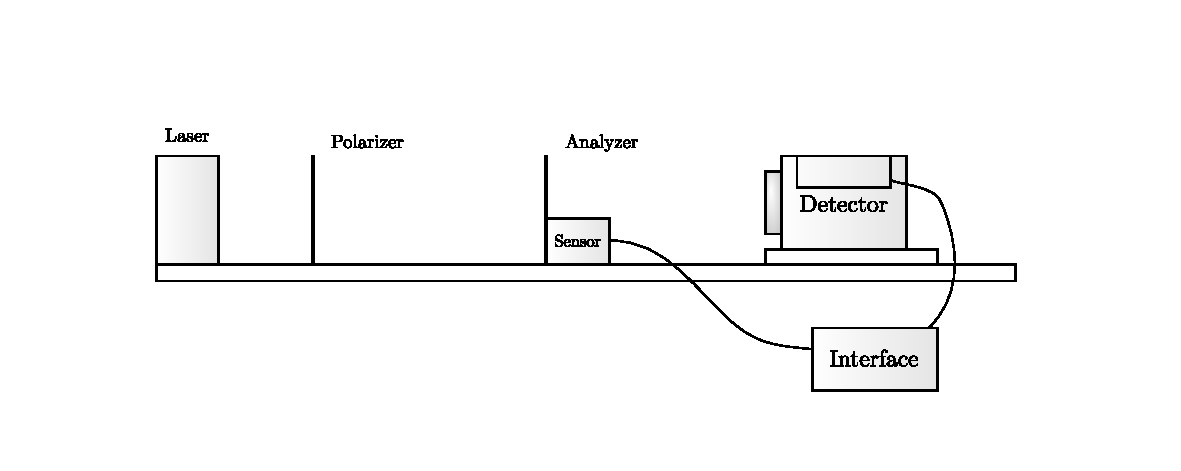
\includegraphics[scale=0.6]{figures/f1.pdf}
  \caption{Experimental setup.}
  \label{fig:1}
\end{figure}

Let's denote the angle between the axis of the first polarizer and axis of the analyzer as $\theta$. If the intensity of the light before passing the analyzer is $I_0$, and the intensity of the light after passing the analyzer is $I$, then the Malu's law states that the intensity of the light after passing the analyzer is given by the equation\cite[]{Hecht_2017}
\begin{equation}
  I = I_{in}\left[H_{90}+\left(H_0-H_{90}\right)\right]
  \label{eq:1}
\end{equation}

The procedure of the experiment as follows. First, we turn on the laser and adjust the polarizers so that their axes are parallel. Next, we turn on the interface, namely Pasco\textsuperscript{\textregistered} Xplorer GLX, and start the data collection. We rotate the analyezer by 400\degree. Then we stop the data collection and conclude the experiment.

\section{Data \& Results}
After extracting the data and plotting it using Python, we obtained the following plot of the intensity of the light after passing the analyzer as a function of the angle between the axes of the polarizer and the analyzer (see Figure \ref{fig:2}).
Plot appears to be in form of a sinusoidal function. After fitting to data using Python again it can observed that best fit line is in form of $I(\theta) = a + b\cos^2(\theta)$ (see Figure \ref{fig:3}), or more precisely:
\begin{equation}
  I(\theta) = 2.3271\cos^2(1.001\cdot\theta+1.42)
  \label{eq:2}
\end{equation}
\begin{figure}[ht]
  \centering
  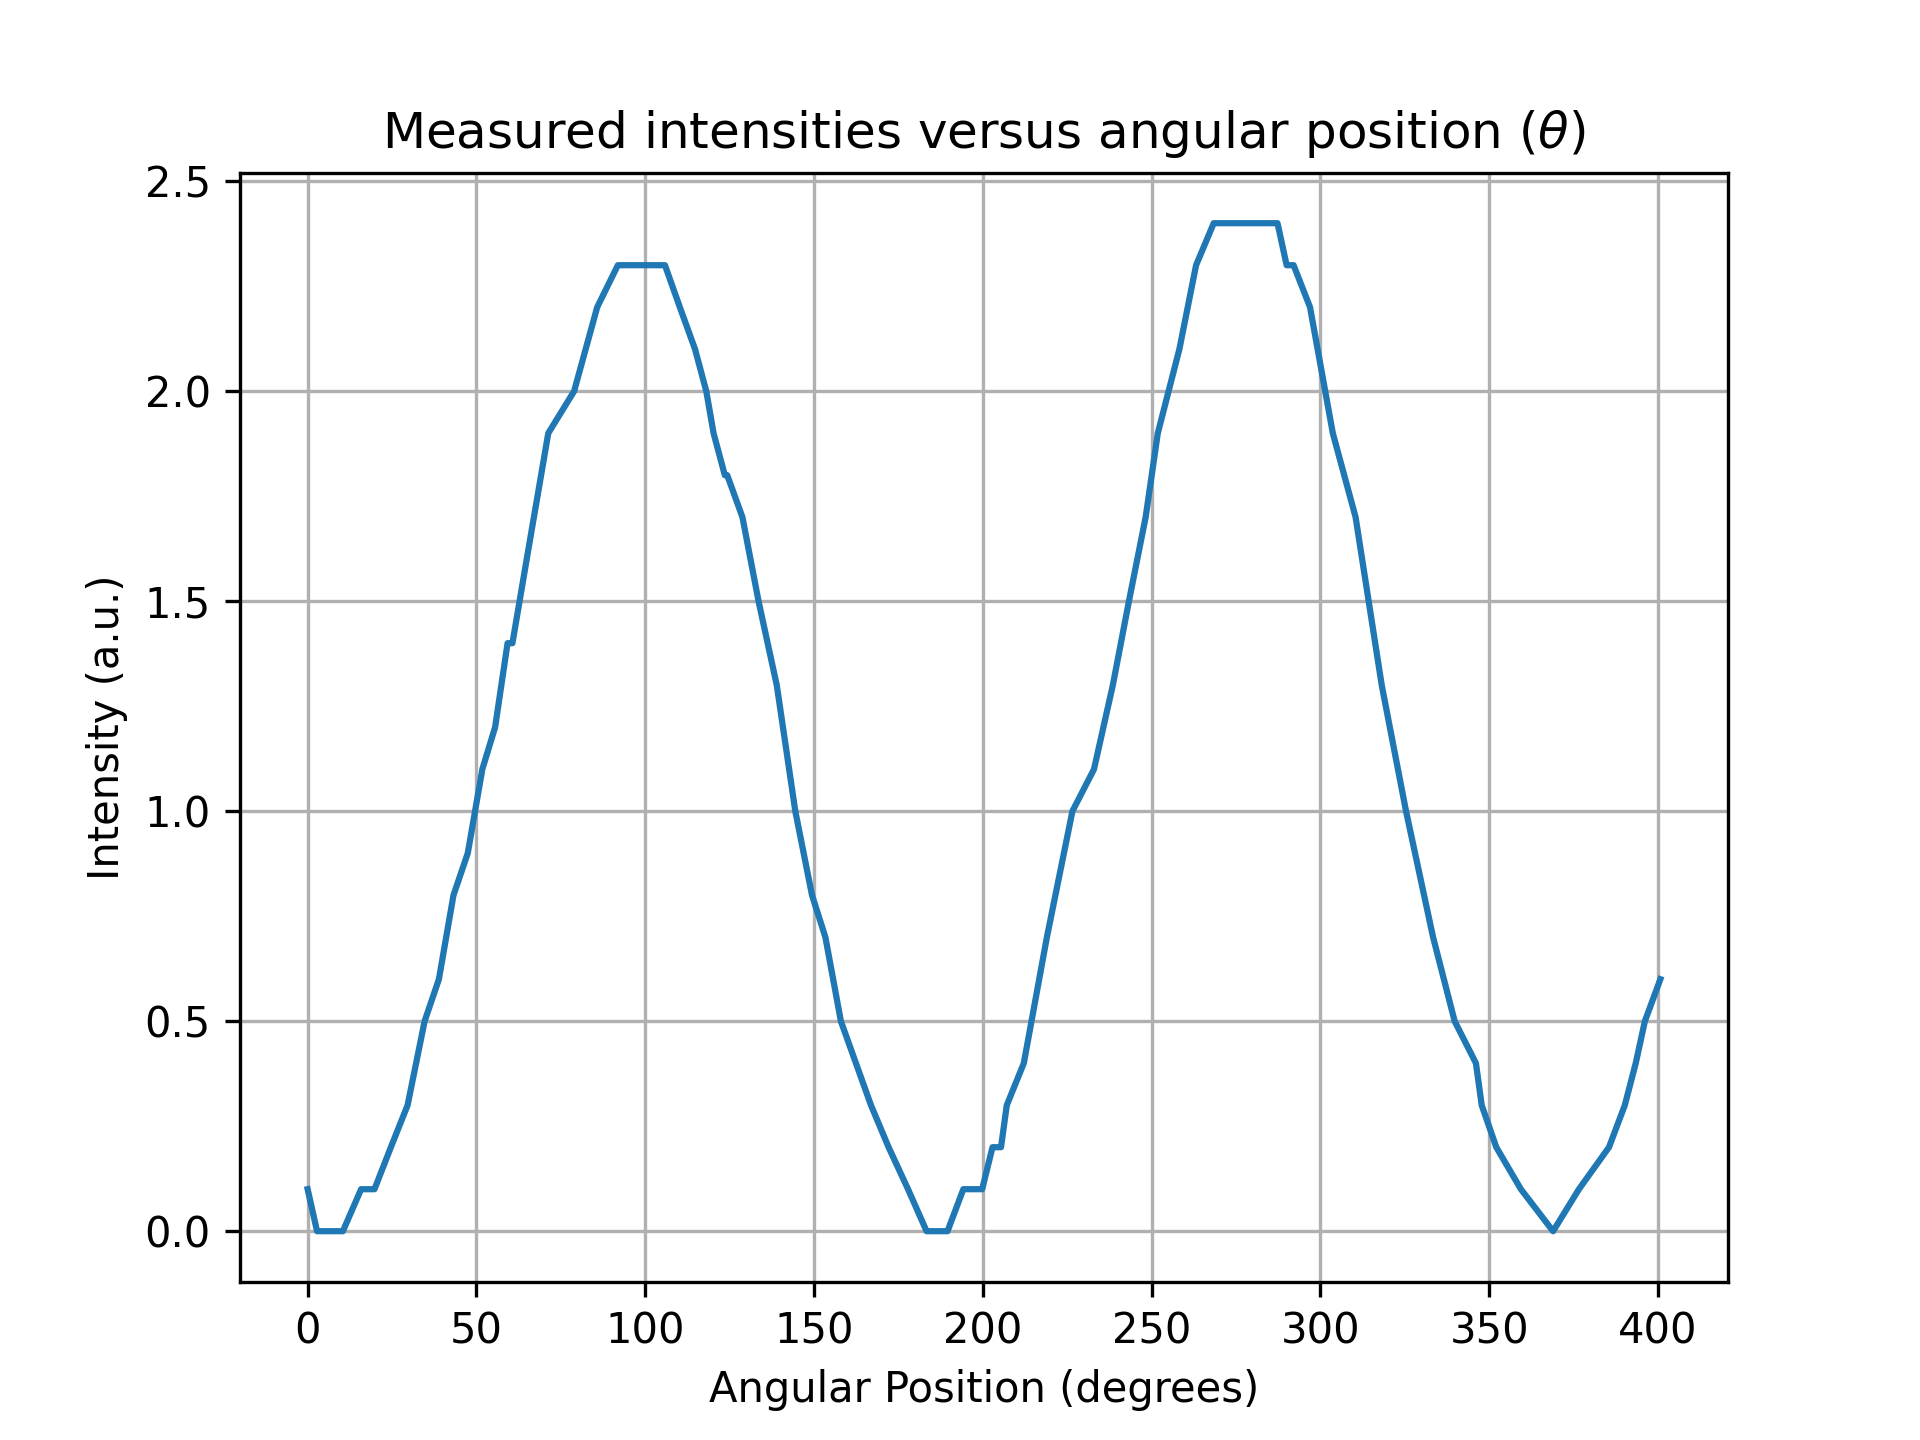
\includegraphics[scale=0.6]{plots/plot1.png}
  \caption{Plot of the intensity of the light after passing the analyzer as a function of the angle between the axes of the polarizer and the analyzer.}
  \label{fig:2}
\end{figure}

\begin{figure}[ht]
  \centering
  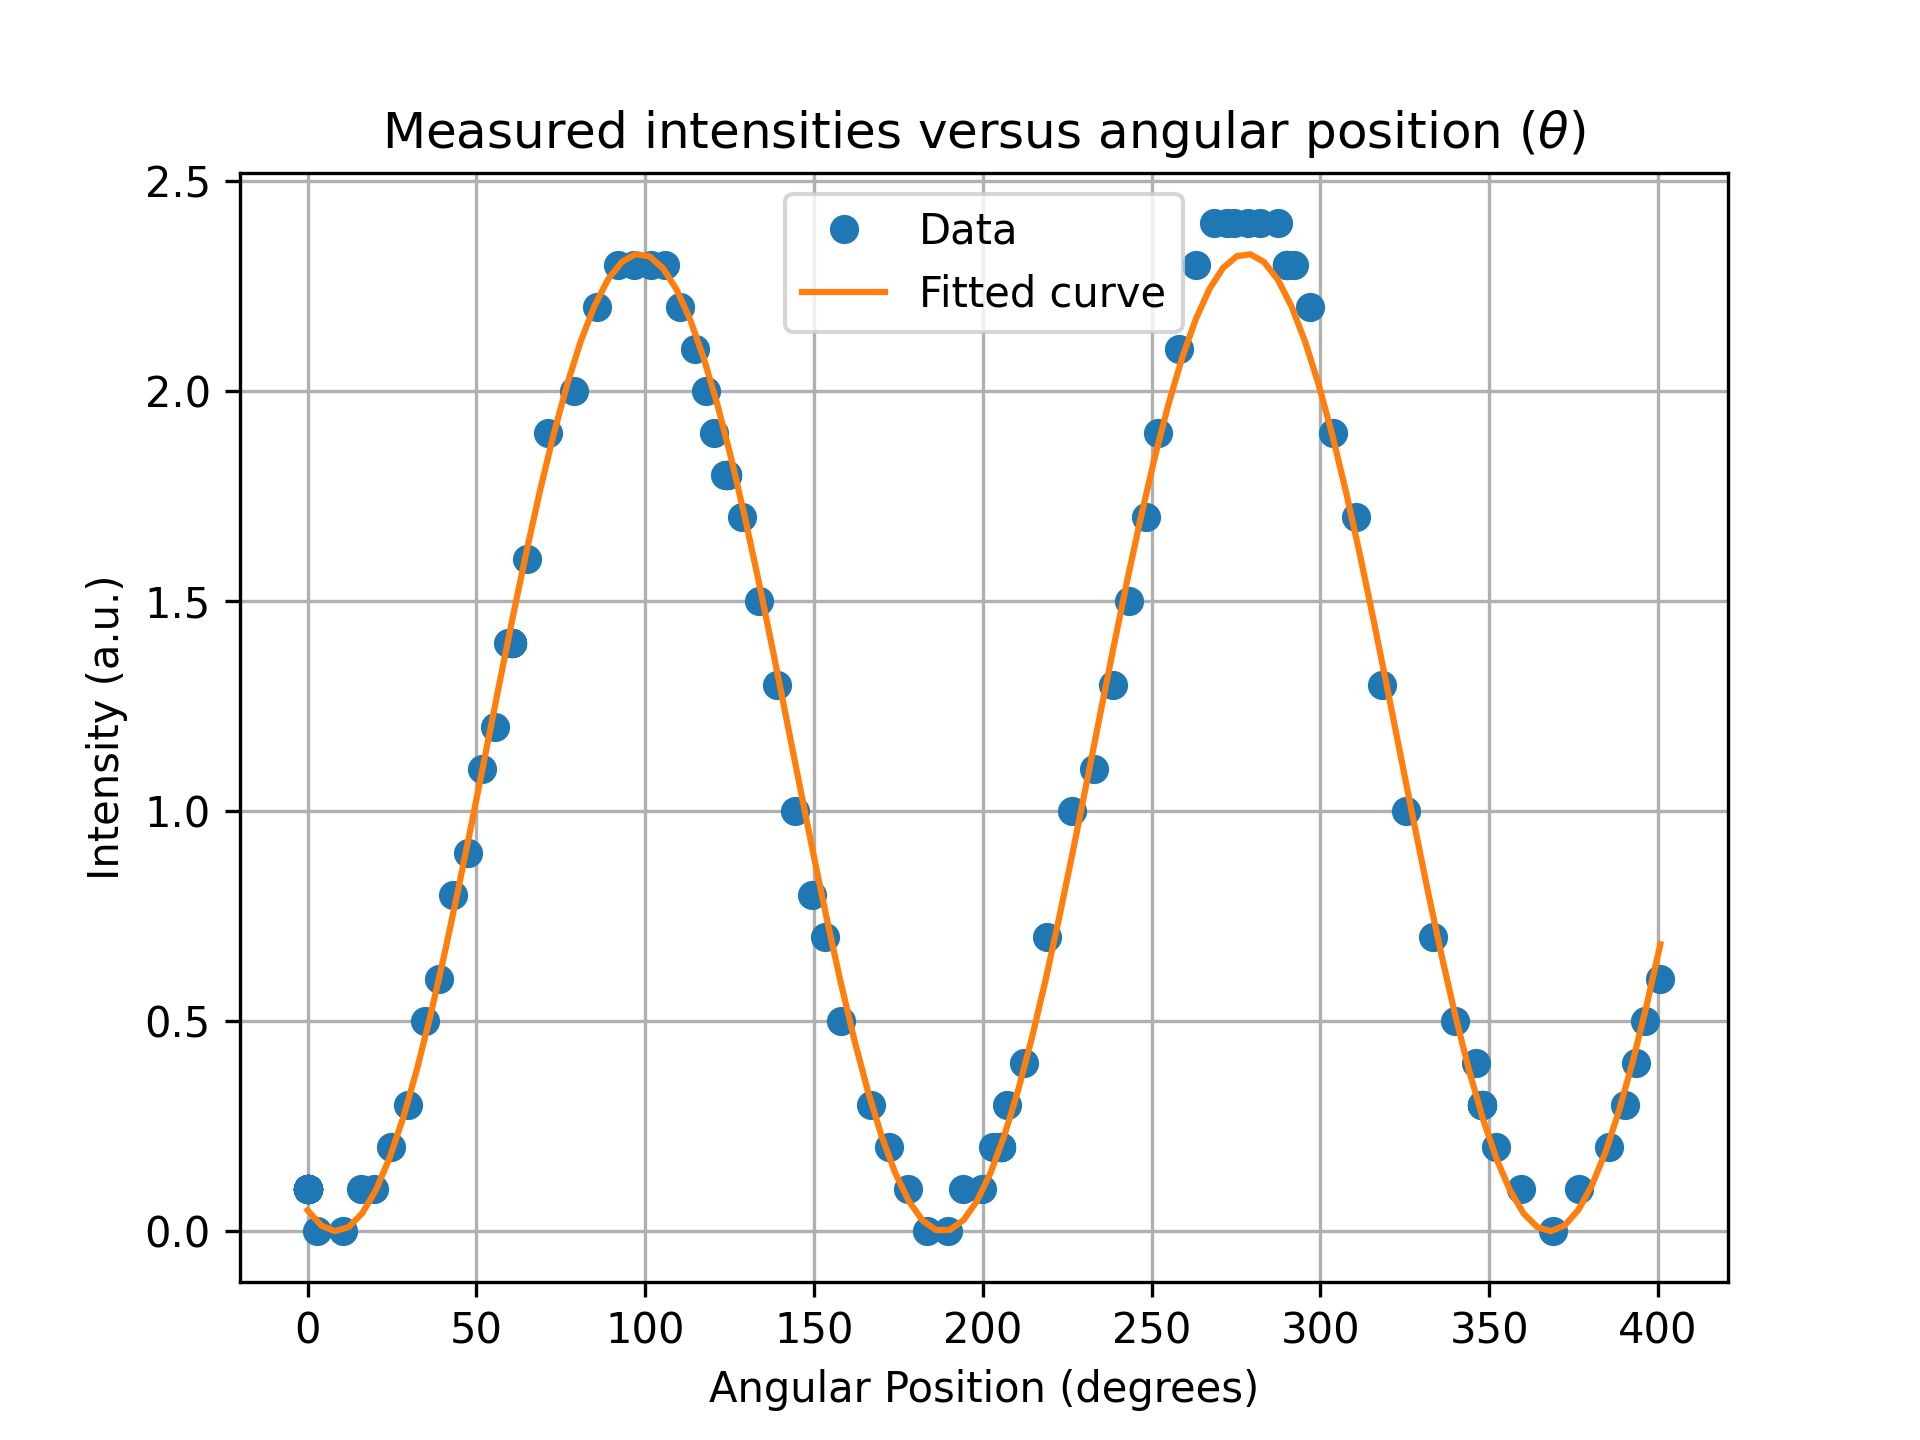
\includegraphics[scale=0.6]{plots/plot2.png}
  \caption{Best fit of the data to the Malu's law.}
  \label{fig:3}
\end{figure}
Which tells us that the Malu's law is verified, and also suggests that our incident light is linearly polarized.
 
\section{Discussion \& Conclusion}
Due to computerized nature of this experiment, error is minimized. However, there are still some sources of error. First one being manual allignment of polarizers at the start of the experiment, which is the reason for phase shift in the best fit line. Another point of error is manual rotation of the analyzer, which wasn't uniform is the reason behind the fluctations at some points, and also higher density of points in some regions that others.

Anotther point of error lies in best fit line. It being best fit line, it is not the exact representation of the data. However due to more than 100 data points we can fairly assume that it is close to the real value.

In conclusion, experiment was successful in verifying the Malu's law, and also in determining that the incident light is linearly polarized, and also was fully in line with the theory.
\printbibliography

\end{document}